\documentclass[english,11pt, reqno, oneside]{amsart}
\usepackage{amsmath}
\usepackage{amssymb}
\usepackage[usenames,dvipsnames]{xcolor}
\usepackage[colorlinks=true,linkcolor=blue!95!black, citecolor = green!55!black,bookmarksdepth=3]{hyperref}
\usepackage{tikz}
\usetikzlibrary{calc}
\usetikzlibrary{math}
\usetikzlibrary{decorations.markings, decorations.pathreplacing,shapes.misc}

\begin{document}

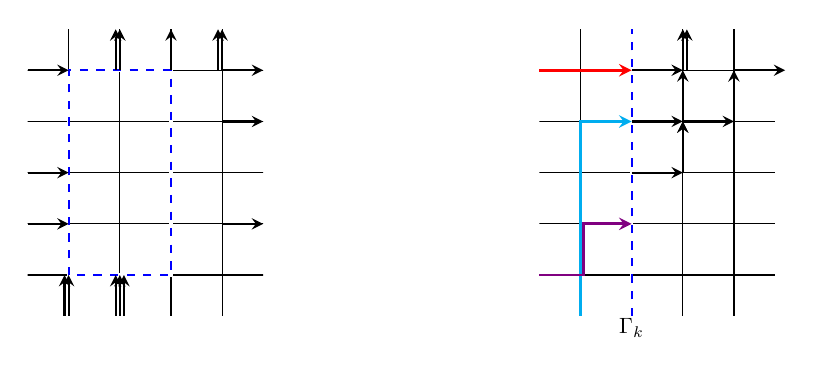
\begin{tikzpicture}[scale=1.3]




% RIGHT PANEL
\begin{scope}[shift={(5,0)}]
\begin{scope}
\clip (-0.4, -0.4) rectangle (1.9, 2.4);
\draw (-1,-1) grid[step=0.5] (3,3);
\end{scope}

\draw[white, very thick] (0.5, -0.4) -- ++(0,2.8);
\draw[dashed, blue, thick] (0.5,-0.4) -- ++(0,2.8);
\node[anchor=north, scale=0.8] at (0.5,-0.35) {$\Gamma_k$};

% left side arrows
\draw[line width=1pt, -stealth, cyan] (0, -0.4) -- ++(0, 1.9) -- ++(0.5,0);
\draw[line width=1pt, -stealth, violet] (-0.4, 0) -- ++(0.43, 0) -- ++(0,0.5) -- ++(0.47,0);
\draw[line width=1pt, -stealth, red] (-0.4, 2) -- ++(0.9,0);


% % horizontal black arrow tips
\foreach \x/\y in {0.5/2, 0.5/1.5, 0.5/1, 1/1.5, 1.5/2}%
  \draw[thick, -stealth] (\x, \y) -- ++(0.5,0);


% % vertical black arrow tips
\foreach \x/\y in {1/1, 1/1.5, 1/1, 1.5/1.5}%
  \draw[thick, -stealth] (\x, \y) -- ++(0, 0.5);

% % top most vertical arrows
\foreach \x/\y in {1/2, 1.04/2}%
  \draw[thick, -stealth] (\x, \y) -- ++(0, 0.4);

\end{scope}




%%%% LEFT PANEL
\begin{scope}
\clip (-0.4, -0.4) rectangle (1.9, 2.4);
\draw (-1,-1) grid[step=0.5] (3,3);
\end{scope}

\draw[white, very thick] (0,0) rectangle (1,2);
\draw[dashed, blue, thick] (0,0) rectangle (1,2);



% top arrows
\foreach \x [count=\c from 6] in {1.46, 1.5, 1, 0.5, 0.46}
  \draw[thick, -stealth] (\x, 2) -- ++(0,0.4);


%bottom arrows
\foreach \x [count=\c] in {-0.04, 0, 0.46, 0.5, 0.54}
  \draw[thick, -stealth] (\x, -0.4) -- ++(0,0.4);


\useasboundingbox (current bounding box);

% right side arrows
\foreach \y [count =\c from 3] in {0.5, 1.5, 2}
  \draw[thick, -stealth] (1.5, \y) --  ++(0.4,0);


% left side arrows
\foreach \y [count =\c from 9] in {2, 1, 0.5}
  \draw[thick, -stealth] (-0.4, \y) -- ++(0.4,0);



\end{tikzpicture}

\end{document}